\documentclass{beamer}
\usepackage{booktabs}
\usepackage[autostyle]{csquotes}
\usepackage{multicol,lipsum,microtype}
% \usepackage[xcdraw,dvipsnames]{xcolor}
% \usepackage[backend=biber]{biblatex}
% \addbibresource{./prensentation.tex/bib/main.bib}
\usepackage{listings}
\usepackage{lstautogobble}  % Fix relative indenting
\usepackage{xargs}
\usepackage{float}
\usepackage{tikz}
\usepackage{bytefield}
\usepackage{pgf-umlsd}
\usepackage{pgfplots}
\pgfplotsset{compat=1.16}
\usepgfplotslibrary{statistics}
\usepgfplotslibrary{groupplots}
\usepackage{caption}
\usepackage{subcaption}
\usepackage{acronym}
\usepackage{mathtools}
\usepackage{amssymb}
\usepackage{amsmath}
\usepackage{zi4}            % Nice font
\usepackage{booktabs}
\usepackage{multirow}
\usepackage{hyperref}
\usepackage[toc,page]{appendix}

\definecolor{bluekeywords}{rgb}{0.13, 0.13, 1}
\definecolor{greencomments}{rgb}{0, 0.5, 0}
\definecolor{redstrings}{rgb}{0.9, 0, 0}
\definecolor{graynumbers}{rgb}{0.5, 0.5, 0.5}

\usepackage[colorinlistoftodos,prependcaption,textsize=tiny]{todonotes}
\newcommandx{\unsure}[2][1=]{\todo[linecolor=red,backgroundcolor=red!25,bordercolor=red,#1]{#2}}
\newcommandx{\change}[2][1=]{\todo[linecolor=blue,backgroundcolor=blue!25,bordercolor=blue,#1]{#2}}
\newcommandx{\info}[2][1=]{\todo[linecolor=OliveGreen,backgroundcolor=OliveGreen!25,bordercolor=OliveGreen,#1]{#2}}
\newcommandx{\improvement}[2][1=]{\todo[linecolor=Plum,backgroundcolor=Plum!25,bordercolor=Plum,#1]{#2}}
\newcommandx{\thiswillnotshow}[2][1=]{\todo[disable,#1]{#2}}

% \usetikzlibrary{external}
% \tikzexternalize[prefix=tikz/]
% \usepackage[a4paper,landscape,hmargin={1cm,1cm}]{geometry}
\usepackage{tikz-timing}[2014/10/29]
\usetikztiminglibrary[rising arrows]{clockarrows}
\usetikzlibrary{fit}
\usetikzlibrary{calc}
\usetikzlibrary{quotes}
\usetikzlibrary{positioning}
\usetikzlibrary{arrows,automata}
\usetikzlibrary{backgrounds,calc,shadings,shadows}
\usepackage{circuitikz}
\usetikzlibrary{shapes,decorations.pathreplacing}

\tikzstyle{bag} = [align=center]

\makeatletter
\pgfkeys{/pgf/.cd,
  parallelepiped offset x/.initial=2mm,
  parallelepiped offset y/.initial=2mm
}
\pgfdeclareshape{parallelepiped}
{
  \inheritsavedanchors[from=rectangle] % this is nearly a rectangle
  \inheritanchorborder[from=rectangle]
  \inheritanchor[from=rectangle]{north}
  \inheritanchor[from=rectangle]{north west}
  \inheritanchor[from=rectangle]{north east}
  \inheritanchor[from=rectangle]{center}
  \inheritanchor[from=rectangle]{west}
  \inheritanchor[from=rectangle]{east}
  \inheritanchor[from=rectangle]{mid}
  \inheritanchor[from=rectangle]{mid west}
  \inheritanchor[from=rectangle]{mid east}
  \inheritanchor[from=rectangle]{base}
  \inheritanchor[from=rectangle]{base west}
  \inheritanchor[from=rectangle]{base east}
  \inheritanchor[from=rectangle]{south}
  \inheritanchor[from=rectangle]{south west}
  \inheritanchor[from=rectangle]{south east}
  \backgroundpath{
    % store lower right in xa/ya and upper right in xb/yb
    \southwest \pgf@xa=\pgf@x \pgf@ya=\pgf@y
    \northeast \pgf@xb=\pgf@x \pgf@yb=\pgf@y
    \pgfmathsetlength\pgfutil@tempdima{\pgfkeysvalueof{/pgf/parallelepiped
      offset x}}
    \pgfmathsetlength\pgfutil@tempdimb{\pgfkeysvalueof{/pgf/parallelepiped
      offset y}}
    \def\ppd@offset{\pgfpoint{\pgfutil@tempdima}{\pgfutil@tempdimb}}
    \pgfpathmoveto{\pgfqpoint{\pgf@xa}{\pgf@ya}}
    \pgfpathlineto{\pgfqpoint{\pgf@xb}{\pgf@ya}}
    \pgfpathlineto{\pgfqpoint{\pgf@xb}{\pgf@yb}}
    \pgfpathlineto{\pgfqpoint{\pgf@xa}{\pgf@yb}}
    \pgfpathclose
    \pgfpathmoveto{\pgfqpoint{\pgf@xb}{\pgf@ya}}
    \pgfpathlineto{\pgfpointadd{\pgfpoint{\pgf@xb}{\pgf@ya}}{\ppd@offset}}
    \pgfpathlineto{\pgfpointadd{\pgfpoint{\pgf@xb}{\pgf@yb}}{\ppd@offset}}
    \pgfpathlineto{\pgfpointadd{\pgfpoint{\pgf@xa}{\pgf@yb}}{\ppd@offset}}
    \pgfpathlineto{\pgfqpoint{\pgf@xa}{\pgf@yb}}
    \pgfpathmoveto{\pgfqpoint{\pgf@xb}{\pgf@yb}}
    \pgfpathlineto{\pgfpointadd{\pgfpoint{\pgf@xb}{\pgf@yb}}{\ppd@offset}}
  }
}
\makeatother

\definecolor{listing-background}{HTML}{F7F7F7}
\definecolor{listing-rule}{HTML}{B3B2B3}
\definecolor{listing-numbers}{HTML}{B3B2B3}
\definecolor{listing-text-color}{HTML}{000000}
\definecolor{listing-keyword}{HTML}{435489}
\definecolor{listing-keyword-2}{HTML}{1284CA} % additional keywords
\definecolor{listing-keyword-3}{HTML}{9137CB} % additional keywords
\definecolor{listing-identifier}{HTML}{435489}
\definecolor{listing-string}{HTML}{00999A}
\definecolor{listing-comment}{HTML}{8E8E8E}

\lstset{
  language         = C++,
  numbers          = left,
  xleftmargin      = 2.7em,
  framexleftmargin = 2.5em,
  backgroundcolor  = \color{listing-background},
  basicstyle       = \color{listing-text-color}\linespread{1.0}\small\ttfamily{},
  breaklines       = true,
  frame            = single,
  framesep         = 0.19em,
  rulecolor        = \color{listing-rule},
  frameround       = ffff,
  tabsize          = 4,
  numberstyle      = \color{listing-numbers},
  aboveskip        = 1.0em,
  belowskip        = 0.1em,
  abovecaptionskip = 0em,
  belowcaptionskip = 1.0em,
  keywordstyle     = {\color{listing-keyword}\bfseries},
  keywordstyle     = {[2]\color{listing-keyword-2}\bfseries},
  keywordstyle     = {[3]\color{listing-keyword-3}\bfseries\itshape},
  sensitive        = true,
  identifierstyle  = \color{listing-identifier},
  commentstyle     = \color{listing-comment},
  stringstyle      = \color{listing-string},
  showstringspaces = false,
  escapeinside     = {/*@}{@*/}, % Allow LaTeX inside these special comments
  literate         =
  {á}{{\'a}}1 {é}{{\'e}}1 {í}{{\'i}}1 {ó}{{\'o}}1 {ú}{{\'u}}1
  {Á}{{\'A}}1 {É}{{\'E}}1 {Í}{{\'I}}1 {Ó}{{\'O}}1 {Ú}{{\'U}}1
  {à}{{\`a}}1 {è}{{\'e}}1 {ì}{{\`i}}1 {ò}{{\`o}}1 {ù}{{\`u}}1
  {À}{{\`A}}1 {È}{{\'E}}1 {Ì}{{\`I}}1 {Ò}{{\`O}}1 {Ù}{{\`U}}1
  {ä}{{\"a}}1 {ë}{{\"e}}1 {ï}{{\"i}}1 {ö}{{\"o}}1 {ü}{{\"u}}1
  {Ä}{{\"A}}1 {Ë}{{\"E}}1 {Ï}{{\"I}}1 {Ö}{{\"O}}1 {Ü}{{\"U}}1
  {â}{{\^a}}1 {ê}{{\^e}}1 {î}{{\^i}}1 {ô}{{\^o}}1 {û}{{\^u}}1
  {Â}{{\^A}}1 {Ê}{{\^E}}1 {Î}{{\^I}}1 {Ô}{{\^O}}1 {Û}{{\^U}}1
  {œ}{{\oe}}1 {Œ}{{\OE}}1 {æ}{{\ae}}1 {Æ}{{\AE}}1 {ß}{{\ss}}1
  {ç}{{\c c}}1 {Ç}{{\c C}}1 {ø}{{\o}}1 {å}{{\r a}}1 {Å}{{\r A}}1
  {€}{{\EUR}}1 {£}{{\pounds}}1 {«}{{\guillemotleft}}1
  {»}{{\guillemotright}}1 {ñ}{{\~n}}1 {Ñ}{{\~N}}1 {¿}{{?`}}1
  {…}{{\ldots}}1 {≥}{{>=}}1 {≤}{{<=}}1 {„}{{\glqq}}1 {“}{{\grqq}}1
  {”}{{''}}1
}
\lstdefinelanguage{none}{
  identifierstyle=,
  commentstyle=,
  stringstyle=,
  keywordstyle=,
}

\def\lav{lavander!90}
\def\oran{orange!30}

\tikzstyle{motes}=[draw,circle,bottom color= gray,
                  top color= white,minimum width=10pt]
\tikzstyle{gateways}=[draw,circle, left color= orange,minimum width=20pt]

\tikzset{l3 switch/.style={
    minimum width=0.75cm,
    minimum height=0.75cm,
    parallelepiped,fill=switch, draw=white,
    parallelepiped offset x=1.75mm,
    parallelepiped offset y=1.25mm,
    path picture={
      \node[fill=white,
        circle,
        minimum size=6pt,
        inner sep=0pt,
        append after command={
          \pgfextra{
            \foreach \angle in {0,45,...,360}
            \draw[-latex,fill=white] (\tikzlastnode.\angle)--++(\angle:2.25mm);
          }
        }
      ]
       at ([xshift=-0.75mm,yshift=-0.5mm]path picture bounding box.center){};
    }
  },
  ports/.style={
    line width=0.3pt,
    top color=gray!20,
    bottom color=gray!80
  },
  rack switch/.style={
    minimum width=1.25cm,
    minimum height=0.25cm,
    parallelepiped,fill=white, draw,
    parallelepiped offset x=2mm,
    parallelepiped offset y=1.25mm,
    xscale=-1,
    path picture={
      \draw[top color=gray!5,bottom color=gray!40]
      (path picture bounding box.south west) rectangle
      (path picture bounding box.north east);
      \coordinate (A-west) at ([xshift=-0.2cm]path picture bounding box.west);
      \coordinate (A-center) at ($(path picture bounding box.center)!0!(path
        picture bounding box.south)$);
      \foreach \x in {0.275,0.525,0.775}{
        \draw[ports]([yshift=-0.05cm]$(A-west)!\x!(A-center)$)
          rectangle +(0.1,0.05);
        \draw[ports]([yshift=-0.125cm]$(A-west)!\x!(A-center)$)
          rectangle +(0.1,0.05);
       }
      \coordinate (A-east) at (path picture bounding box.east);
      \foreach \x in {0.085,0.21,0.335,0.455,0.635,0.755,0.875,1}{
        \draw[ports]([yshift=-0.1125cm]$(A-east)!\x!(A-center)$)
          rectangle +(0.05,0.1);
      }
    }
  },
  server/.style={
    fill=white, draw,
    minimum width=0.35cm,
    minimum height=0.75cm,
    parallelepiped,
    parallelepiped offset x=3mm,
    parallelepiped offset y=2mm,
    xscale=-1,
    path picture={
      \draw[top color=gray!5,bottom color=gray!40]
      (path picture bounding box.south west) rectangle
      (path picture bounding box.north east);
      \coordinate (A-center) at ($(path picture bounding box.center)!0!(path
        picture bounding box.south)$);
      \coordinate (A-west) at ([xshift=-0.575cm]path picture bounding box.west);
      \draw[ports]([yshift=0.1cm]$(A-west)!0!(A-center)$)
        rectangle +(0.2,0.065);
      \draw[ports]([yshift=0.01cm]$(A-west)!0.085!(A-center)$)
        rectangle +(0.15,0.05);
      \fill[black]([yshift=-0.35cm]$(A-west)!-0.1!(A-center)$)
        rectangle +(0.235,0.0175);
      \fill[black]([yshift=-0.385cm]$(A-west)!-0.1!(A-center)$)
        rectangle +(0.235,0.0175);
      \fill[black]([yshift=-0.42cm]$(A-west)!-0.1!(A-center)$)
        rectangle +(0.235,0.0175);
    }
  },
  invisible/.style={opacity=0},
  visible on/.style={alt={#1{}{invisible}}},
  alt/.code args={<#1>#2#3}{%
    \alt<#1>{\pgfkeysalso{#2}}{\pgfkeysalso{#3}} % \pgfkeysalso doesn't change the path
  },
}

\newcommand{\messdash}[4][0]{
  \stepcounter{seqlevel}
  \path
  (#2)+(0,-\theseqlevel*\unitfactor-0.7*\unitfactor) node (mess from) {};
  \addtocounter{seqlevel}{#1}
  \path
  (#4)+(0,-\theseqlevel*\unitfactor-0.7*\unitfactor) node (mess to) {};
  \draw[->,>=angle 60, dashed] (mess from) -- (mess to) node[midway, above]
  {#3};

  \node (#3 from) at (mess from) {};
  \node (#3 to) at (mess to) {};
}




%\usetheme{vub} % This will automatically load all fonts (Roboto and TeX Gyre Adventor
               % for titles), and the VUB colors. Also includes the triangle.
\usetheme[coloredtitles]{vub}
%\usetheme[showsection]{vub}
\title{Enabling~IPv6~multi-hop~networks with~Time Slotted~Channel~Hopping and~long~range~LoRA~radios} % Can be omitted
\subtitle{Promotors: Prof. Dr. Ir. Kris Steenhaut\newline Prof. Dr. Ir. Elisa Gonzalez Boix\newline Supervisor: Roald Van Glabbeek}
\author{Thomas Perale}

\begin{document}
\frame{\maketitle} % Automatic titlepage with VUB logo.

\begin{frame}{Table of Content}
    % We are going to start at a very high level overview to then dig into the
    % more detailled aspect of LoRa.
    \tableofcontents
\end{frame}

\section{Introduction}

{
  \setbeamercolor{background canvas}{bg=vubbleu}
  \setbeamercolor{normal text}{fg=white}
  \usebeamercolor*{normal text}
\begin{frame}[c]{}
  \centering
  \LARGE
  \vubfont
  ~Introduction
\end{frame}
}

\begin{frame}{Introduction}
\framesubtitle{IoT}
\begin{columns}
\begin{column}{0.6\textwidth}
\begin{itemize}
  \item 25 billion devices connected
  \item Analytics, management
  \item Multiple Sectors
  \begin{itemize}
    \item Transportation
    \item Smart city
    \item Smart domotics
    \item Smart health
    \item Supply Chain
    \item Agriculture
    \item \ldots
  \end{itemize}
\end{itemize}
\end{column}
\begin{column}{0.4\textwidth}
\begin{figure}
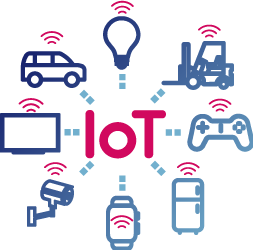
\includegraphics[width=0.8\textwidth]{presentation.tex/fig/iot.png}
\end{figure}
\end{column}
\end{columns}
\end{frame}

\begin{frame}{Introduction}
\framesubtitle{Low Power Wide Area Network (LPWAN)}

\begin{columns}
\begin{column}{0.3\textwidth}
\only<1>{
Short-range
\begin{itemize}
    \item Low power
    \item Small range
    \item Low cost
    \item Low data-rate
    % \item Built for IoT
\end{itemize}
}
\only<2>{
WiFi
\begin{itemize}
    \item Small range
    \item High data-rate
\end{itemize}
}
\only<3>{
Cellular
\begin{itemize}
    \item Long range
    \item High deployement cost
    \item High data-rate
\end{itemize}
}
\only<4>{
LPWAN
\begin{itemize}
    \item Low power
    \item Long range
    \item Low cost
    \item Low data-rate
    \item Built for IoT
    % \begin{itemize}
    %     \item Large scale monitoring
    %     \item Battery operated
    % \end{itemize}
\end{itemize}
}
\end{column}
\begin{column}{0.7\textwidth}

\begin{figure}[H] % TODO More info on axis
\centering
  \resizebox{7.8cm}{4cm}{%
  \begin{tikzpicture}
    \draw[->,thick] (-0.1,0)--(12,0) node[right]{Range};
    \draw[->,thick] (0,-0.1)--(0,8) node[above]{Data Rate};
    \node[] at (1, -0.5) {10m};
    \draw[] (1,-0.1)--(1,0.1);
    \node[] at (3, -0.5) {100m};
    \draw[] (3,-0.1)--(3,0.1);
    \node[] at (5, -0.5) {1km};
    \draw[] (5,-0.1)--(5,0.1);
    \node[] at (7, -0.5) {10km};
    \draw[] (7,-0.1)--(7,0.1);
    \node[] at (9, -0.5) {100km};
    \draw[] (9,-0.1)--(9,0.1);

    \node[] at (-1.2, 1) {1 kbit/sec};
    \draw[] (-0.1,1)--(0.1,1);
    \node[] at (-1.2, 3) {1 Mbit/sec};
    \draw[] (-0.1,3)--(0.1,3);
    \node[] at (-1.2, 5) {100 Mbit/sec};
    \draw[] (-0.1,5)--(0.1,5);
    \node[] at (-1.2, 7) {1 Gbit/sec};
    \draw[] (-0.1,7)--(0.1,7);

    \only<4->{
    \node[draw,fill=white, visible on=<4->] at (8,1.5) (lora) {LoRa};
    \node[draw,fill=white, visible on=<4->] at (8.7,0.8) (sigfox) {SigFox};
    \node[draw,fill=white, visible on=<4->] at (7.4,2.2) (nb) {NB-IOT};
    \begin{scope}[on background layer]
      \node[draw,fill=blue!30,fit=(lora) (sigfox) (nb), label=above:{LPWAN}, visible on=<4->] {};
    \end{scope}
    }

    \node[draw,fill=white] at (2.2,3.5) (bluetooth) {Bluetooth};
    \node[draw,fill=white] at (2.7,2.5) (zigbee) {ZigBee};
    \node[draw,fill=white] at (2.0,1.8) (ble) {BLE};
    \begin{scope}[on background layer]
      \node[draw,fill=blue!10,fit=(bluetooth) (zigbee) (ble), label=above:{Short-range}] {};
    \end{scope}

    \only<2->{
    \node[draw,fill=white, visible on=<2->] at (3,5) (wifi) {WiFi};
    \begin{scope}[on background layer]
      \node[draw,fill=blue!50,fit=(wifi), visible on=<2->] {};
    \end{scope}
    }

    \only<3->{
    \node[draw,fill=white, visible on=<3->] at (6.8,5) (lte) {LTE};
    \node[draw,fill=white, visible on=<3->] at (5.8,6) (5g) {5G};
    \begin{scope}[on background layer]
      \node[draw,fill=blue!60,fit=(lte) (5g), label=above:{Cellular}, visible on=<3->] {};
    \end{scope}
    }

    \node[] at (6.9,8.2) (leg5) {\small Low};
    \node[draw,fill=blue!10] at (7.5,8.2) (leg1) {};
    \node[draw,fill=blue!30] at (7.8,8.2) (leg2) {};
    \node[draw,fill=blue!50] at (8.1,8.2) (leg3) {};
    \node[draw,fill=blue!60] at (8.4,8.2) (leg4) {};
    \node[] at (10.7,8.2) (leg5) {\small High Power Consumption};
\end{tikzpicture}
  }
\caption{Comparison of IoT technologies}
\label{fig:commrangegraph}
\end{figure}
\end{column}
\end{columns}
\end{frame}

\begin{frame}{Introduction}
\framesubtitle{LoRa}
\begin{itemize}
  \item 
\end{itemize}
\end{frame}

\begin{frame}{Introduction}
\framesubtitle{LoRaWAN}
\begin{columns}
\begin{column}{0.5\textwidth}
\begin{itemize}
    \item Stars-of-stars topology
    \begin{itemize}
      \item End-nodes/Motes
      \item Gateways
      \item Central Server
    \end{itemize}
    \item Direct Link to gateway
    \item Transmit as soon as possible
    \begin{itemize}
      \item Low channel occupation
      \item Power efficient
    \end{itemize}
\end{itemize}
\end{column}
\begin{column}{0.5\textwidth}
\begin{figure}[H]
    \centering
    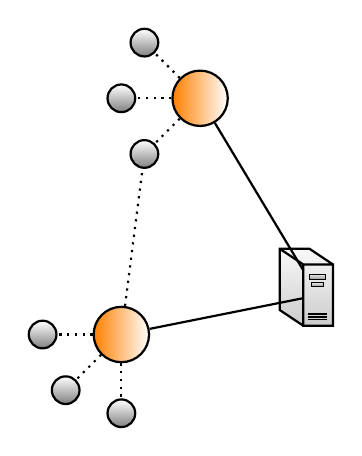
\begin{tikzpicture}[auto, thick]
      % Place super peers and connect them
      \foreach \place/\name in {{(-1,-2)/a}, {(-0,1)/b}}
        \node[gateways] (\name) at \place {};
      \node[server] (d) at (1.5,-1.5) {};
      %
      \foreach \source/\dest in {a/d, b/d}
        \path[] (\source) edge (\dest);

      % Place normal peers
      \foreach \pos/\i in {above left of/1, left of/2, below left of/3}
        \node[motes, \pos =b ] (b\i) {};
      \foreach \speer/\peer in {b/b1,b/b2,b/b3}
        \path[dotted] (\speer) edge (\peer);
      %
      \foreach \pos/\i in {below left of/1, below of/2, left of/3}
        \node[motes, \pos =a ] (a\i) {};
      \foreach \speer/\peer in {a/a1,a/a2,a/a3}
        \path[dotted] (\speer) edge (\peer);
      %
      \path[dotted] (a) edge (b3);
    \end{tikzpicture}
    \caption{Star topology\label{fig:startopology}}
\end{figure}
\end{column}
\end{columns}
\end{frame}





\section{Problem}

{
  \setbeamercolor{background canvas}{bg=vubbleu}
  \setbeamercolor{normal text}{fg=white}
  \usebeamercolor*{normal text}
\begin{frame}[c]{}
  \centering
  \LARGE
  \vubfont
  ~Problem
\end{frame}
}

\begin{frame}{Problem}
\framesubtitle{LoRaWAN - Does Not Scale}
\begin{columns}
\begin{column}{0.4\textwidth}
\begin{itemize}
    \item No channel sensing
    \begin{itemize}
        \item Collision
    \end{itemize}
    \item SF7 Over-usage
    \item Duty-cycle limitation
    \begin{itemize}
        \item 36 sec of transmission/hour
    \end{itemize}
\end{itemize}
\end{column}
\begin{column}{0.6\textwidth}
\begin{figure}[H] % TODO More info on axis
\centering
  \resizebox{7cm}{4cm}{%

  \begin{tikzpicture}[
    description/.style={draw, rectangle},
    arr/.style={help lines,black!70,<->},
    zigzag/.style={to path={ -- ($(\tikztostart)!.55!-7:(\tikztotarget)$) -- ($(\tikztostart)!.45!7:(\tikztotarget)$) -- (\tikztotarget) \tikztonodes}}
    ]
    \draw[->,thick] (-0.1,0)--(12,0) node[right]{time};
    \draw[->,thick] (0,-0.1)--(0,8) node[above]{};

    \node[] at (-1.2, 2) {Node 1};
    \draw[] (-0.1,2)--(0.1,2);
    \only<2->{
    \node[] at (-1.2, 6) {Node 2};
    \draw[] (-0.1,6)--(0.1,6);
    }

    \draw[] (0.5,1)--(0.5,3);
    \node[] at (1, 0.5) {Wake up};
    \only<2->{
    \draw[] (3.5,5)--(3.5,7);
    \node[] at (3.5, 4.5) {Wake up};
    }

    \begin{scope}[xshift=0cm,yshift=0cm,inner sep=0pt, outer sep=0pt]
        \only<2->{
        \begin{scope}[on background layer]
            \node[draw,fill=gray!10,fit={(4,5) (6,7)}] {};
            \node[draw,fill=blue!10,fit={(6,5) (12,7)}] {};
        \end{scope}
        \node () [description, fit={(4,5) (6,7)}, label=center:{Preamble}] {};
        \node () [description, fit={(6,5) (12,7)}, label=center:{Payload}] {};
        }

        \begin{scope}[on background layer]
            \node[draw,fill=gray!10,fit={(1,1) (3,3)}] {};
            \node[draw,fill=blue!10,fit={(3,1) (10,3)}] {};
        \end{scope}
        \node () [description, fit={(1,1) (3,3)}, label=center:{Preamble}] {};
        \node () [description, fit={(3,1) (10,3)}, label=center:{Payload}] {};
    \end{scope}
    \only<3->{
     \draw[-stealth,line width=1mm] (8,5) to[zigzag] +(0,-2);
     \node[] at (9.2, 4.3) {Collision};
    }
\end{tikzpicture}
  }
\caption{Collision between nodes\label{fig:collision}}
\end{figure}

\end{column}
\end{columns}
\end{frame}

\begin{frame}{Problem}
\framesubtitle{LoRaWAN - Coverage}
\begin{columns}
\begin{column}{0.4\textwidth}
\begin{itemize}
   \item Coverage
    \begin{itemize}
        \item Topology
        \item Environmental Factor
    \end{itemize}
    \only<2->{
        \item Bordering node
        \begin{itemize}
            \item High SF
            \item Longer transmission
            \item Higher power consumption
        \end{itemize}
    }
\end{itemize}
\end{column}
\begin{column}{0.6\textwidth}
\begin{figure}[H]
    \centering
    \def\angle{0}
    \def\radius{3}
    \resizebox{4cm}{4cm}{%
    \begin{tikzpicture}[nodes = {font=\sffamily}]
      \foreach \color in {
            yellow,
            red,
            yellow,
            white,
            red,
            yellow,
            white,
            yellow,
            white,
            white,
            red,
            red,
        } {
        \ifx\color\empty\else
            \draw[fill={\color!50},draw={\color}] (0,0) -- (\angle:\radius)
              arc (\angle:\angle+30:\radius) -- cycle;
            \pgfmathparse{\angle+30}
            \xdef\angle{\pgfmathresult}
        \fi
        };
        \xdef\radius{2.5}
        \foreach \color in {
            yellow,
            red,
            yellow,
            yellow,
            red,
            white,
            yellow,
            red,
            white,
            white,
            white,
            white,
        } {
        \ifx\color\empty\else
            \draw[fill={\color!50},draw={\color}] (0,0) -- (\angle:\radius)
              arc (\angle:\angle+30:\radius) -- cycle;
            \pgfmathparse{\angle+30}
            \xdef\angle{\pgfmathresult}
        \fi
        };
        \xdef\radius{2}
        \foreach \color in {
            yellow,
            red,
            green,
            red,
            yellow,
            white,
            yellow,
            white,
            white,
            white,
            white,
            white,
        } {
        \ifx\color\empty\else
            \draw[fill={\color!50},draw={\color}] (0,0) -- (\angle:\radius)
              arc (\angle:\angle+30:\radius) -- cycle;
            \pgfmathparse{\angle+30}
            \xdef\angle{\pgfmathresult}
        \fi
        };
        \xdef\radius{1.5}
        \foreach \color in {
            yellow,
            red,
            yellow,
            yellow,
            yellow,
            green,
            yellow,
            white,
            red,
            white,
            white,
            white,
        } {
        \ifx\color\empty\else
            \draw[fill={\color!50},draw={\color}] (0,0) -- (\angle:\radius)
              arc (\angle:\angle+30:\radius) -- cycle;
            \pgfmathparse{\angle+30}
            \xdef\angle{\pgfmathresult}
        \fi
        };
        \xdef\radius{1}
        \foreach \color in {
            green,
            green,
            green,
            yellow,
            yellow,
            yellow,
            white,
            white,
            yellow,
            red,
            yellow,
            red,
        } {
        \ifx\color\empty\else
            \draw[fill={\color!50},draw={\color}] (0,0) -- (\angle:\radius)
              arc (\angle:\angle+30:\radius) -- cycle;
            \pgfmathparse{\angle+30}
            \xdef\angle{\pgfmathresult}
        \fi
        };
        \xdef\radius{0.5}
        \foreach \color in {
            green,
            green,
            yellow,
            yellow,
            green,
            green,
            yellow,
            red,
            yellow,
            green,
            green,
            green,
        } {
        \ifx\color\empty\else
            \draw[fill={\color!50},dotted,draw={\color}] (0,0) -- (\angle:\radius)
              arc (\angle:\angle+30:\radius) -- cycle;
            \pgfmathparse{\angle+30}
            \xdef\angle{\pgfmathresult}
        \fi
        };
        \only<2->{
            \path[thick, dotted] (-0.7, -1.1) edge (0,0);
            \node[motes] () at (-0.7, -1.1) {};
            \path[thick, dotted] (-1.5, 2.2) edge (0,0);
            \node[motes] () at (-1.5, 2.2) {};
            \path[thick, dotted] (2.5, 2.3) edge (0,0);
            \node[motes] () at (2.5, 2.3) {};
            \path[thick, dotted] (2.2, -2.1) edge (0,0);
            \node[motes] () at (2.2, -2.1) {};
        }
        \foreach \place/\name in {{(0,0)/a}}
            \node[gateways] (\name) at \place {};
    \end{tikzpicture}
    }
\caption{Typical gateway coverage\cite{lorajambalaya}\label{fig:coverage}}
\resizebox{5.5cm}{0.5cm}{%
\begin{tabular}{r@{: }l r@{: }l}

\begin{tikzpicture}\draw[fill=green,line width=1pt]  circle(1ex);\end{tikzpicture} & Good\ Connection & 
\begin{tikzpicture}\draw[fill=yellow,line width=1pt]  circle(1ex);\end{tikzpicture} & Intermediate\ Connection\\

\begin{tikzpicture}\draw[fill=red,line width=1pt]  circle(1ex);\end{tikzpicture} & Bad\ Connection & 
\begin{tikzpicture}\draw[fill=white,line width=1pt]  circle(1ex);\end{tikzpicture} & No\ Connection 
\end{tabular}
}
\end{figure}

\end{column}
\end{columns}
\end{frame}

\begin{frame}{Problem}
\framesubtitle{LoRaWAN - Linear Sensor Network}
\begin{columns}
\begin{column}{0.4\textwidth}
\begin{itemize}
    \item Linear networks
    \begin{itemize}
        \item Pipeline
        \item Tunnels
    \end{itemize}
    \item Expensive infrastructure
    \item Little coverage
\end{itemize}
\end{column}
\begin{column}{0.6\textwidth}

\begin{figure}[H]
    \centering
    \resizebox{6.5cm}{4cm}{%
    \begin{tikzpicture}
    \foreach \place/\name in {{(0,0)/a}}
    \path[->] (-5,0) edge (5,0);
    \node[motes] (a4) at (-4.5, 0) {};
    \node[motes] (a5) at (-2.5, 0) {};
    \node[motes] (a7) at (2.5, 0) {};
    \node[motes] (a8) at (4.5, 0) {};
    \node[gateways] (a) at (0,0) {};
    \draw[dotted,draw={black}] (0,0) circle (3cm);
    \pgfmathparse{\angle+30}
    \xdef\angle{\pgfmathresult}
    \end{tikzpicture}
    }
    \caption{Gateway coverage on linear networks\label{fig:lsn}}
\end{figure}

\end{column}
\end{columns}
\end{frame}

\begin{frame}{Problem}
\framesubtitle{Multi-hop}
\begin{columns}
\begin{column}{0.6\textwidth}
\begin{itemize}
    \item Message relayed to neighbor
    \item Range increased
    \item Power efficient for border nodes
    \item Adapt to topology
    \item Overall higher energy consumption
\end{itemize}
\end{column}
\begin{column}{0.4\textwidth}
\begin{figure}[H]
    \centering
    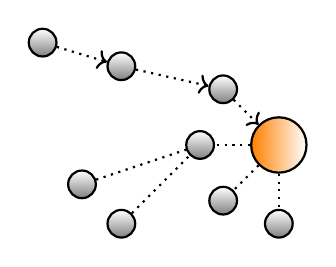
\begin{tikzpicture}[auto, thick]
      % Place super peers and connect them
      \foreach \place/\name in {{(0,0)/a}}
        \node[gateways] (\name) at \place {};
      \node[motes] (a4) at (-2, 1) {};
      \node[motes] (a5) at (-3, 1.3) {};
      \node[motes] (a7) at (-2.5, -0.5) {};
      \node[motes] (a8) at (-2, -1) {};
     \foreach \pos/\i in {below left of/1, below of/2, left of/3, above left of/6}
        \node[motes, \pos =a ] (a\i) {};
      \foreach \speer/\peer in {a/a1,a/a2,a/a3,a7/a3,a8/a3}
        \path[dotted] (\speer) edge (\peer);
      \path[dotted,->] (a5) edge (a4);
      \path[dotted,->] (a4) edge (a6);
      \path[dotted,->] (a6) edge (a);
    \end{tikzpicture}
    \caption{Multi-hop Communication\label{fig:multihop}}
\end{figure}

\end{column}
\end{columns}

\end{frame}

\begin{frame}{Problem}
\framesubtitle{LoRa Multi-hop Network}
\begin{itemize}
    \item 
\end{itemize}
\end{frame}

\begin{frame}{Problem}
\framesubtitle{Related Work}
\begin{itemize}
    \item 
\end{itemize}
\end{frame}

\begin{frame}{Problem}
\framesubtitle{LoRa Multi-hop Network}
\begin{itemize}
    \item Low-power
    \begin{itemize}
        \item Time-Division
    \end{itemize}
    \item Reliable
    \begin{itemize}
        \item No collision
        \item Interference resistance
        \item Frequency-Division
    \end{itemize}
\end{itemize}
\end{frame}




\section{Approach}

{
  \setbeamercolor{background canvas}{bg=vubbleu}
  \setbeamercolor{normal text}{fg=white}
  \usebeamercolor*{normal text}
\begin{frame}[c]{}
  \centering
  \LARGE
  \vubfont
  ~~Approach
\end{frame}
}

\begin{frame}{Approach}
\framesubtitle{Multihop Routing}

\begin{itemize}
    \item Implementation already exists
    \begin{itemize}
        \item RPL
    \end{itemize}
    \item No guaranty on
    \begin{itemize}
        \item Power efficiency
        \item Reliability
    \end{itemize}
    \item Lack of MAC protocol
\end{itemize}
\end{frame}

\begin{frame}{Approach}
\framesubtitle{Time Slotted Channel Hopping (TSCH)}

\begin{columns}
\begin{column}{0.5\textwidth}

Made for IEEE802.15.4 Phy

\begin{itemize}
  \item Time Division Multiplexing
  \begin{itemize}
    \item Power Efficient
    \item No collision
  \end{itemize}
  \only<2->{
  \item Frequency Division Multiplexing
  \begin{itemize}
    \item External interference resilience
    \item Concurrent transmission
  \end{itemize}
  }
\end{itemize}

\end{column}
\begin{column}{0.5\textwidth}

\begin{figure}[H]
\centering

  \resizebox{5cm}{4cm}{%
  \begin{tikzpicture}[
    asn/.style={black!70, minimum size=1cm},
    timeslot/.style={draw, rectangle, minimum size=1cm},
    arr/.style={help lines,black!70,<->},
    desc/.style={black!70},
  ]
    \only<2->{
    \foreach [evaluate={\ts=int(mod(\i, 4))}] \i in {0,...,7} {
    \node (ts3\i) [timeslot] at (\i, 3) {};
    }
    \foreach [evaluate={\ts=int(mod(\i, 4))}] \i in {0,...,7} {
    \node (ts2\i) [timeslot] at (\i, 2) {};
    }
    }
    \foreach [evaluate={\ts=int(mod(\i, 4))}] \i in {0,...,7} {
    \node (ts1\i) [timeslot] at (\i, 1) {};
    }
    \foreach [evaluate={\ts=int(mod(\i, 4))}] \i in {0,...,7} {
    \node (ts\i) [asn] at (\i, 0) {$TS_{\ts}$};
    }

    \only<2->{
    \node (choff3) [black!70] at (-1.5, 3) {$Ch_{off} 2$};
    \node (choff2) [black!70] at (-1.5, 2) {$Ch_{off} 1$};
    \node (choff1) [black!70] at (-1.5, 1) {$Ch_{off} 0$};
    }

    \begin{scope}[on background layer]
    \only<2->{
    \fill[green!50] (ts22.south west) rectangle (ts22.north east);
    \fill[green!50] (ts36.south west) rectangle (ts36.north east);

    \fill[orange!50] (ts30.south west) rectangle (ts30.north east);
    \fill[orange!50] (ts14.south west) rectangle (ts14.north east);

    \fill[blue!50] (ts24.south west) rectangle (ts24.north east);
    }

    \fill[blue!50] (ts10.south west) rectangle (ts10.north east);
    \end{scope}

    \only<2->{
        \draw[ultra thick]
        (ts10.south west) rectangle (ts33.north east)
        (ts14.south west) rectangle (ts37.north east);
    }
    \only<1>{
        \draw[ultra thick]
        (ts10.south west) rectangle (ts13.north east)
        (ts14.south west) rectangle (ts17.north east);
    }

    \draw[arr,->]
    ([yshift=-10pt]ts0.south west) -- node[fill=white] {$time$} ([yshift=-10pt]{ts7.south east});

  \begin{scope}[xshift=2.5cm,yshift=-3cm,->,>=stealth',shorten >=1pt,auto,node distance=2.5cm]
    \tikzstyle{every state}=[thick,draw=gray!50,fill=gray!20,draw=none,text=black]

    \node[state]         (A) [] {A};
    \node[state]         (B) [below of=A]       {B};
    \node[state]         (C) [right of=B]       {C};

    \only<2-> {
      \path (A) edge [bend left,draw=orange!50] node[draw=orange!50] {$TS_1$} (C)
          (B) edge [bend left,draw=blue!50] node[draw=blue!50] {$TS_1$} (A)
          (C) edge [bend left,draw=green!50] node[above right,draw=green!50] {$TS_3$} (A);
    }
    \only<1> {
      \path (B) edge [bend left,draw=blue!50] node[draw=blue!50] {$TS_1$} (A);
    }
  \end{scope}
\end{tikzpicture}
}
\caption{TSCH Schedule\label{fig:customsched}}
\end{figure}
\end{column}
\end{columns}
\end{frame}

\begin{frame}{Approach}
\framesubtitle{TSCH - Time Slots}

\resizebox{11.2cm}{3.8cm}{%
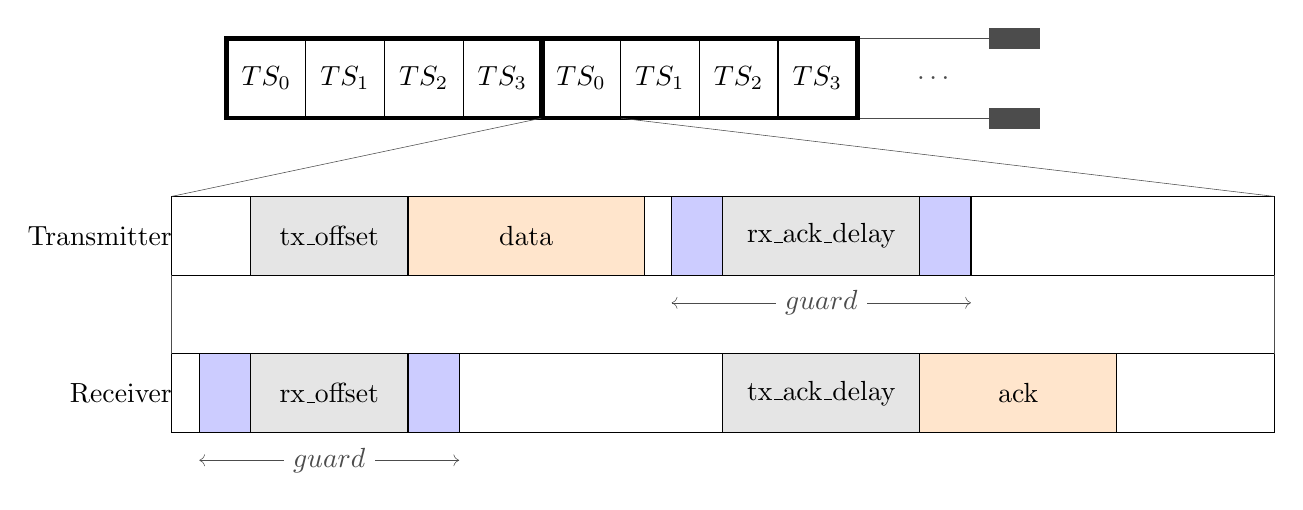
\begin{tikzpicture}[
  timeslot/.style={draw, rectangle, minimum size=1cm},
  description/.style={draw, rectangle, minimum size=1cm},
  arr/.style={help lines,black!70,<->},
]

\foreach [evaluate={\ts=int(mod(\i, 4))}] \i in {0,...,7} {
  \node (ts\i) [timeslot] at (\i, 0) {$TS_{\ts}$};
}
\node (ts8) [minimum height=1cm, minimum width=2cm, black!70] at (8.5, 0) {\ldots};

\draw[help lines, black!70]
  (ts8.north west) -- (ts8.north east) node[fill=white, black!70] {$\ldots$};
\draw[help lines, black!70]
  (ts8.south west) -- (ts8.south east) node[fill=white, black!70] {$\ldots$};

\draw[ultra thick] 
  (ts0.south west) rectangle (ts3.north east)
  (ts4.south west) rectangle (ts7.north east);

\begin{scope}[xshift=-1.2cm,yshift=-2.5cm,inner sep=0pt, outer sep=0pt]
  \node (desc) [draw,rectangle,fit={(0,0) (14,1)}, label=left:{Transmitter~}] {};
  \node (desc1) [description, fill=orange!20, fit={(3,0) (6,1)}, label=center:{data}] {};
  \node (desc0) [description, fill=gray!20, fit={(1,0) (3,1)}, label=center:{tx\_offset}] {};
  \node (descsync1) [description, fill=blue!20, fit={(6.7,0) (7,1)}] {};
  \node (descsync2) [description, fill=blue!20, fit={(9.5,0) (9.8,1)}] {};
  \node (desc2) [description, fill=gray!20, fit={(7,0) (9.5,1)}, label=center:{rx\_ack\_delay}] {};
\end{scope}

\draw[help lines, black!70,-]
  ([yshift=0pt]ts4.south west) -- 
  ([yshift=0pt]{desc.north west});
\draw[help lines, black!70,-]
  ([yshift=0pt]ts4.south east) -- 
  ([yshift=0pt]{desc.north east});

\begin{scope}[xshift=-1.2cm,yshift=-4.5cm,inner sep=0pt, outer sep=0pt]
  \node (ddesc) [draw,rectangle,fit={(0,0) (14,1)}, label=left:{Receiver~}] {};
  \node (ddescsync1) [description, fill=blue!20, fit={(0.7,0) (1,1)}] {};
  \node (ddescsync2) [description, fill=blue!20, fit={(3,0) (3.3,1)}] {};
  \node (ddesc0) [description, fill=gray!20, fit={(1,0) (3,1)}, label=center:{rx\_offset}] {};
  \node (ddesc2) [description, fill=gray!20, fit={(7,0) (9.5,1)}, label=center:{tx\_ack\_delay}] {};
  \node (ddesc3) [description, fill=orange!20, fit={(9.5,0) (12,1)}, label=center:{ack}] {};
\end{scope}

\draw[help lines, black!70,-]
    (desc.south west) -- ({ddesc.north west});
\draw[help lines, black!70,-]
    (desc.south east) -- ({ddesc.north east});

\draw[arr,<->]
    ([yshift=-10pt]descsync1.south west) -- node[fill=white] {$guard$} ([yshift=-10pt]{descsync2.south east});
\draw[arr,<->]
    ([yshift=-10pt]ddescsync1.south west) -- node[fill=white] {$guard$} ([yshift=-10pt]{ddescsync2.south east});

\end{tikzpicture}
}
\end{frame}

\begin{frame}{Approach}
\framesubtitle{TSCH - Channel Hopping}

\begin{itemize}
    \item 
\end{itemize}
\end{frame}

\begin{frame}{Approach}
\framesubtitle{Porting TSCH}

\begin{itemize}
    \item No implementation for LoRa
\end{itemize}
\end{frame}


\section{Test and Validation}

{
  \setbeamercolor{background canvas}{bg=vubbleu}
  \setbeamercolor{normal text}{fg=white}
  \usebeamercolor*{normal text}
\begin{frame}[c]{}
  \centering
  \LARGE
  \vubfont
  ~Test and Validation
\end{frame}
}

\begin{frame}{Realization}
\framesubtitle{Setup}
\begin{columns}
\begin{column}{0.5\textwidth}

\begin{figure}[H]
    \centering
    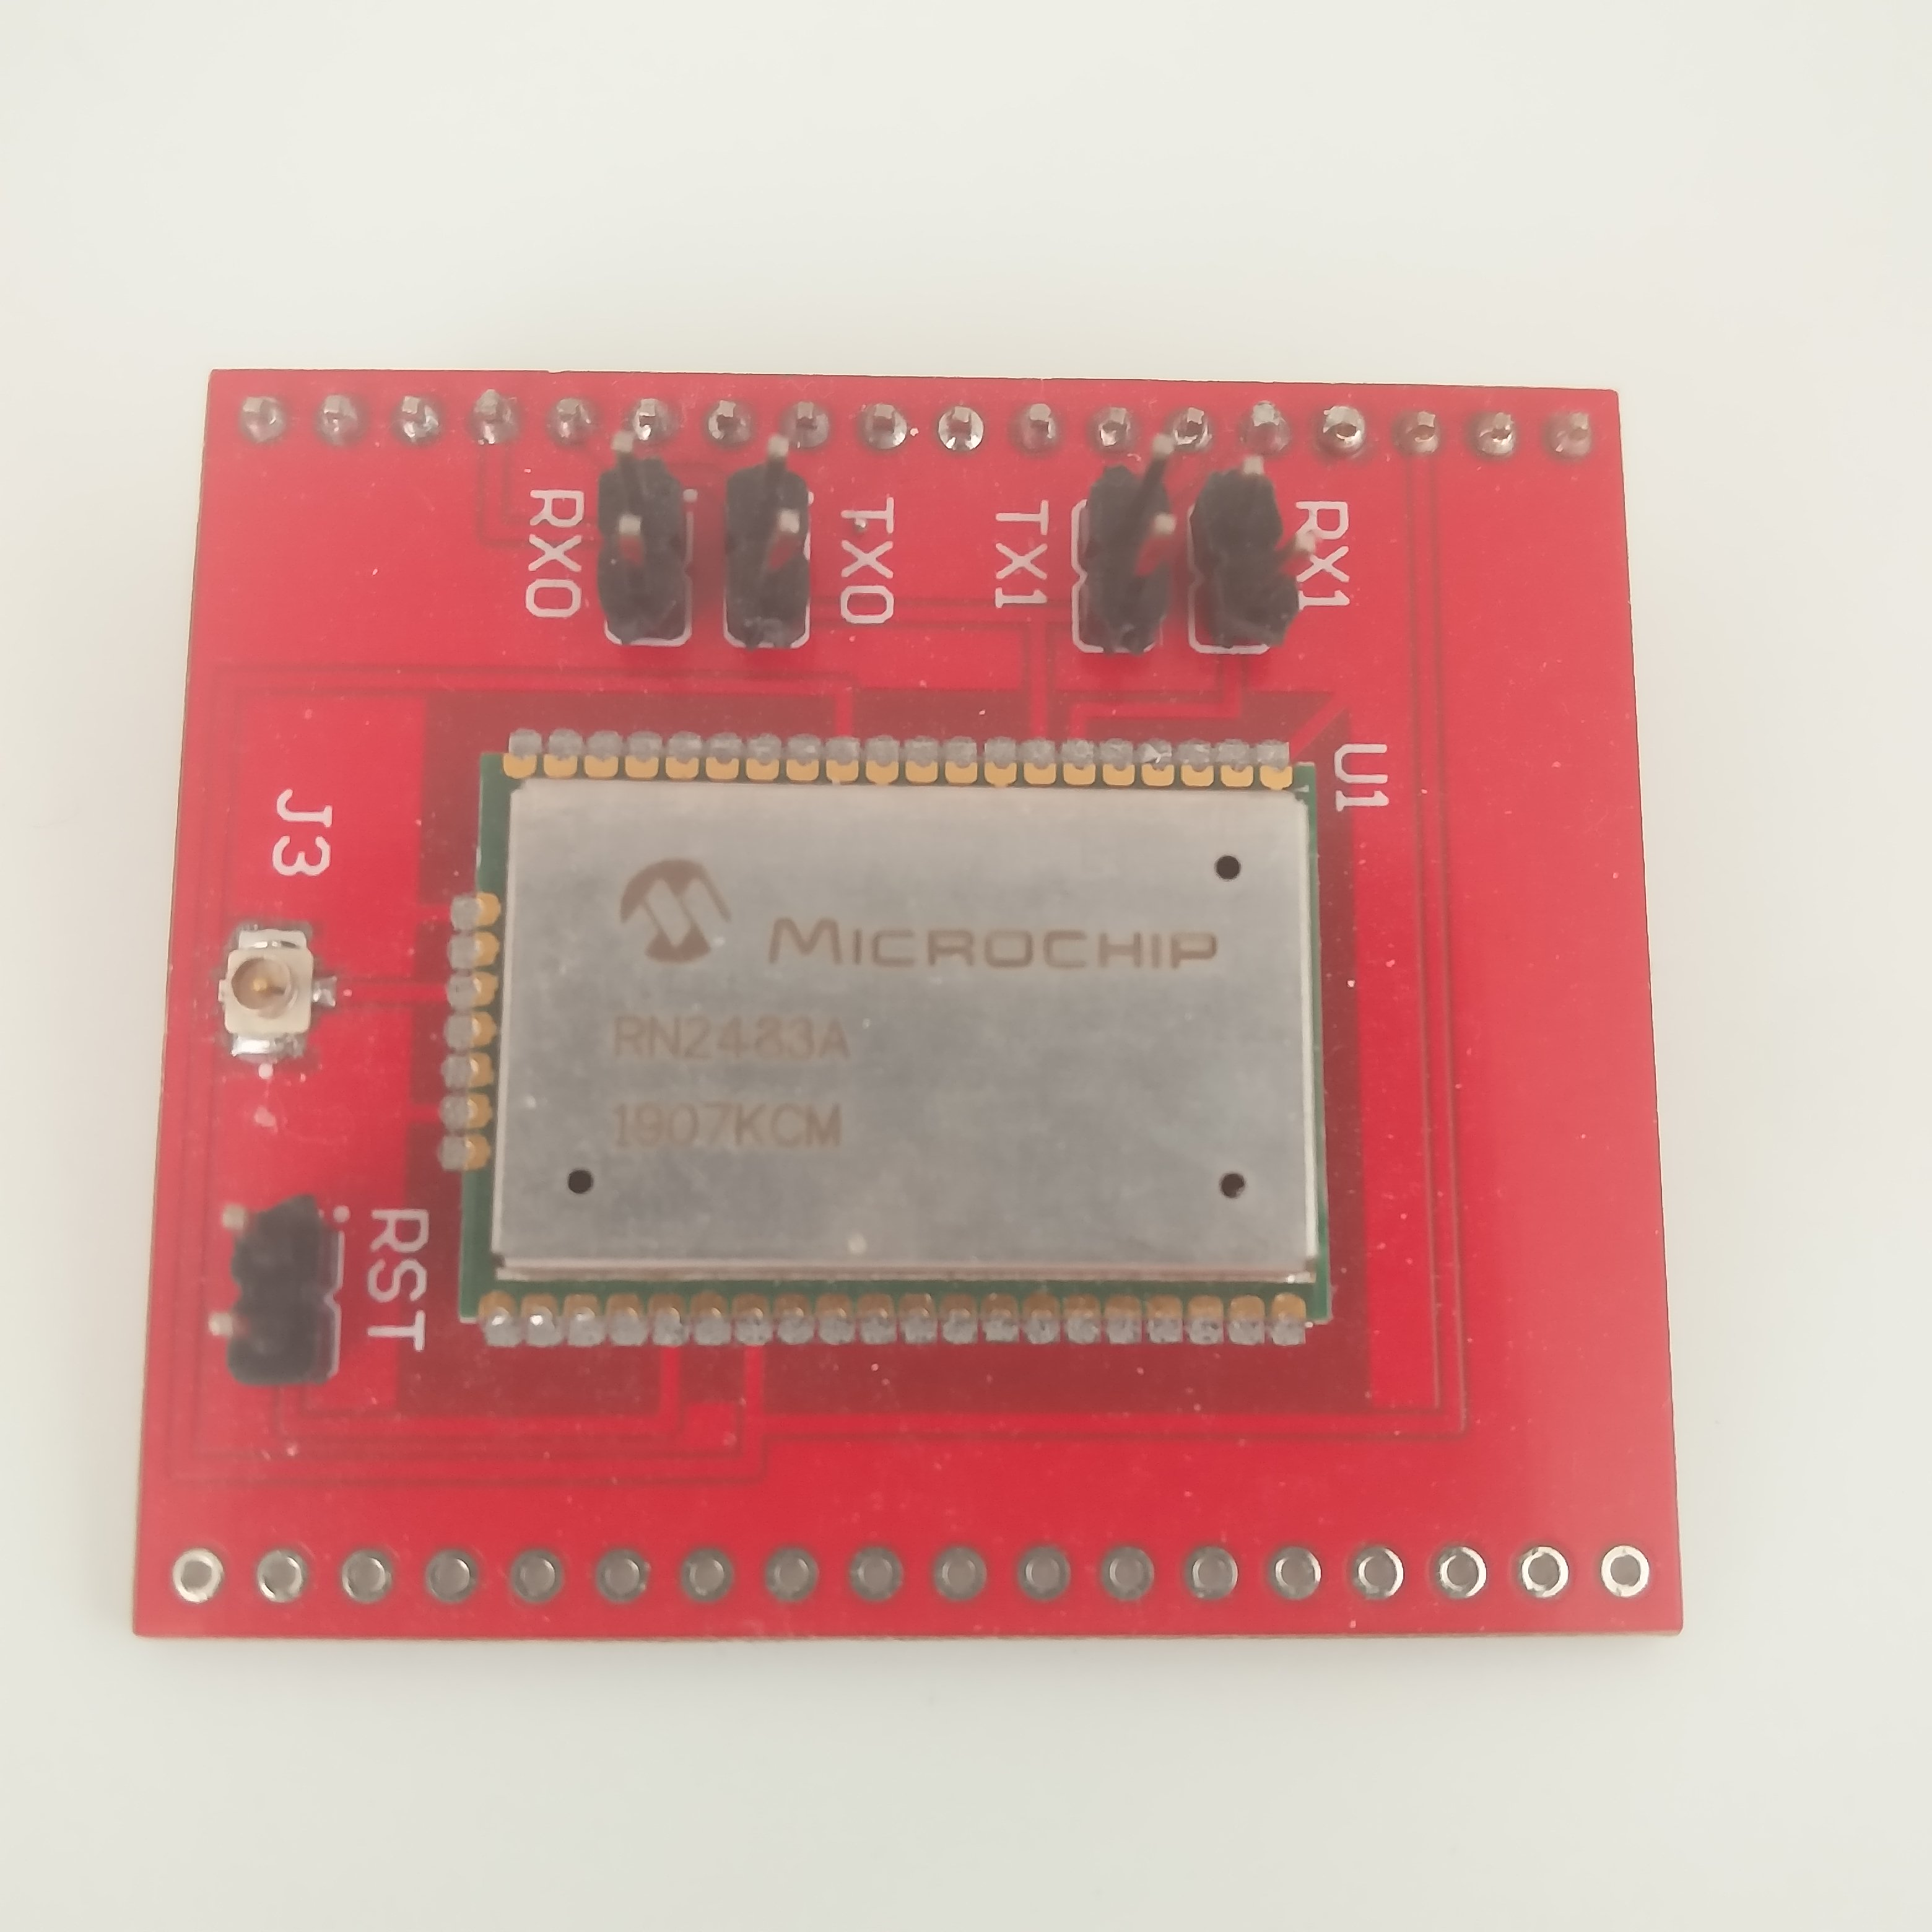
\includegraphics[width=0.6\textwidth]{presentation.tex/fig/rn2483.jpg}
    \caption{The RN2483 LoRa radio shield\label{fig:rn2483pic}}
\end{figure}
\end{column}
\begin{column}{0.5\textwidth}
\begin{figure}[H]
    \centering
    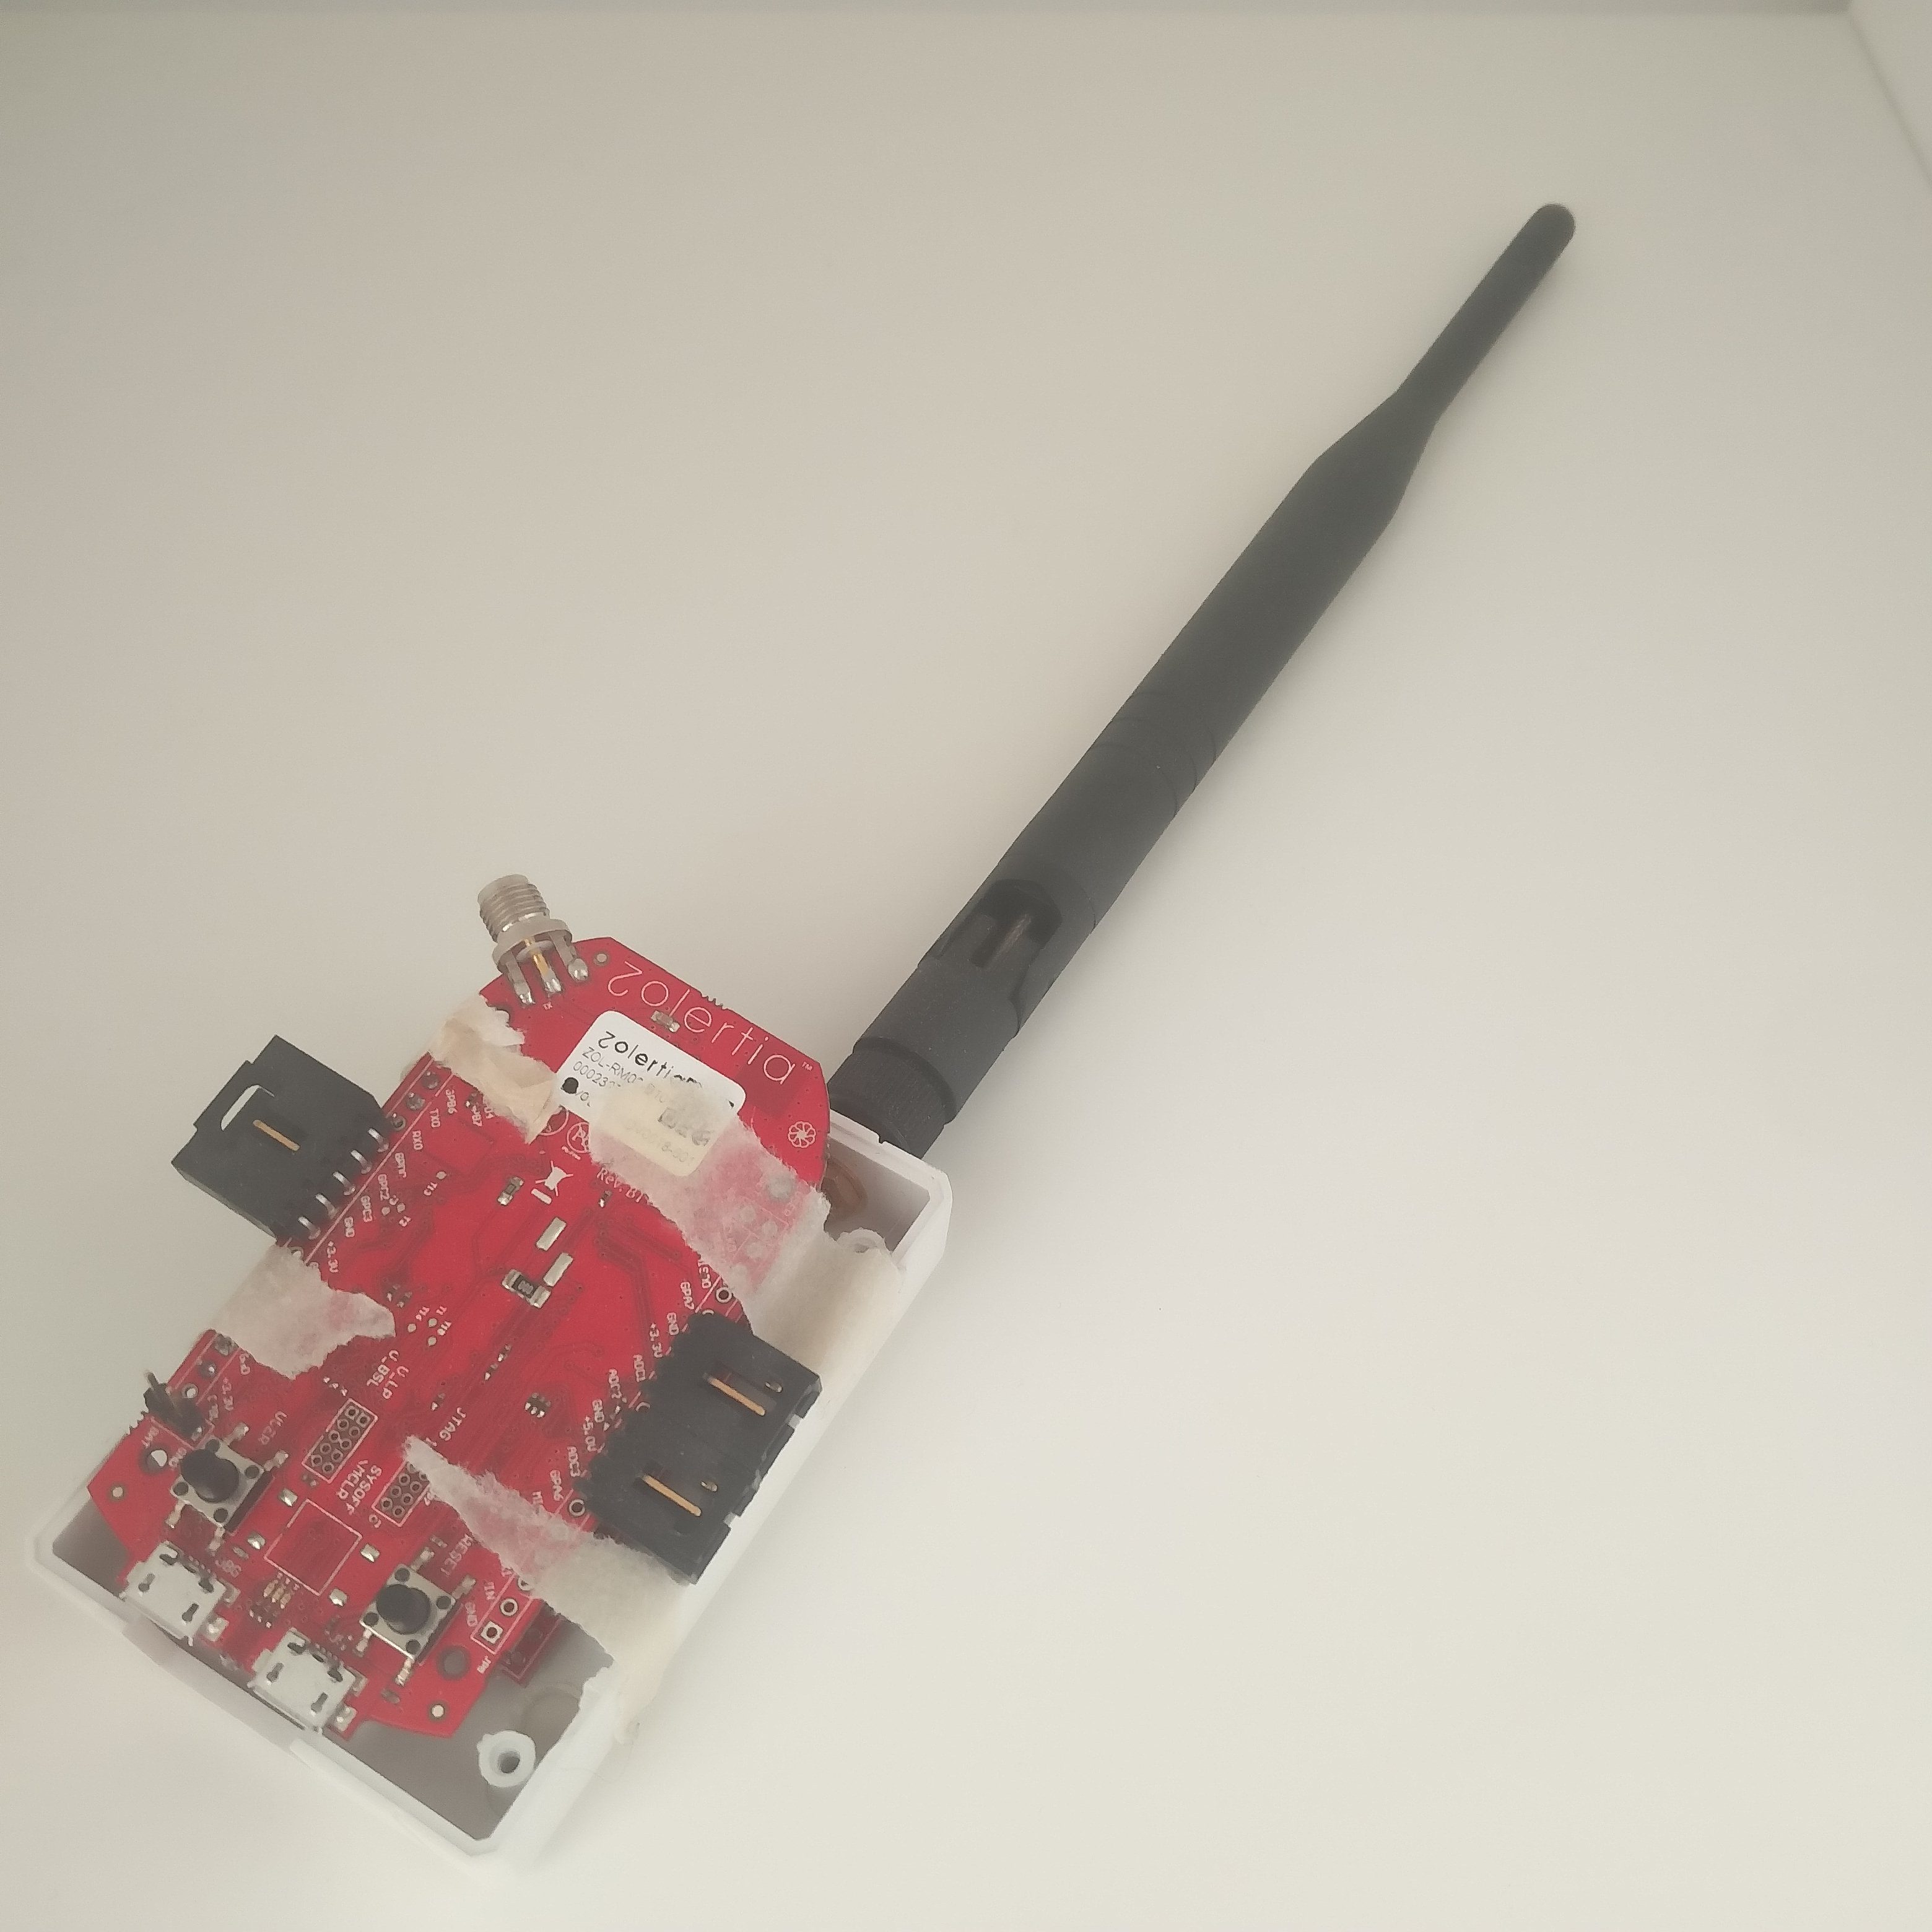
\includegraphics[width=0.6\textwidth]{presentation.tex/fig/zolertia.jpg}
    \caption{The Zolertia RE-Mote with the shield\label{fig:zolpic}}
\end{figure}
\end{column}
\end{columns}
\end{frame}

\begin{frame}{Realization}
\framesubtitle{Driver}

\begin{columns}
\begin{column}{0.5\textwidth}
\begin{itemize}
    \item No LoRa Driver available
    \item Contiki Radio Driver
    \item Syncronized UART communications
\end{itemize}
\end{column}
\begin{column}{0.5\textwidth}
\begin{figure}[H]
\centering
\resizebox{4.6cm}{5.3cm}{%
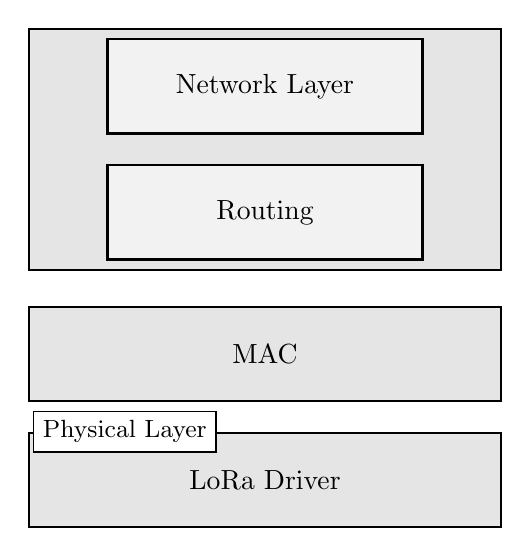
\begin{tikzpicture}[->,>=stealth',shorten >=1pt,auto,node distance=1.6cm]
\tikzstyle{comment}=[
  right=2pt,
  font=\small,
  fill=white,
  text=black,
  draw=black,
]

\tikzstyle{every state}=[rectangle,thick,
  draw=black,fill=gray!20,text=black,
  minimum width= 6cm,
  minimum height= 1.20cm
]

\tikzstyle{smallstate}=[rectangle,thick,
  draw=black,fill=gray!10,text=black,
  minimum width= 4cm,
  minimum height= 1.20cm
]

\node[smallstate]         (A)                    {Network Layer};
\node[smallstate]         (B) [below of=A]       {Routing};
\begin{scope}[on background layer]
  \node[state, fit=(A)(B)] (AB)                 {};
\end{scope}
\node[state,below=1cm]         (C) [below of=AB]       {MAC};
\node[state]         (D) [below of=C]       {LoRa Driver};

\node[comment]       at (D.north west) {Physical Layer};
\end{tikzpicture}
}
\end{figure}
\end{column}
\end{columns}
\end{frame}

\begin{frame}{Realization}
\framesubtitle{Adapt TSCH for LoRa}
\begin{columns}
\begin{column}{0.5\textwidth}
TSCH for LoRa porting issues
\begin{itemize}
    \item Time slot parts timing 
    \item Adaptation to 64bits
    \item Interrupt clash
    \item Watchdog
\end{itemize}
\end{column}
\begin{column}{0.5\textwidth}

\resizebox{5.6cm}{2.3cm}{%
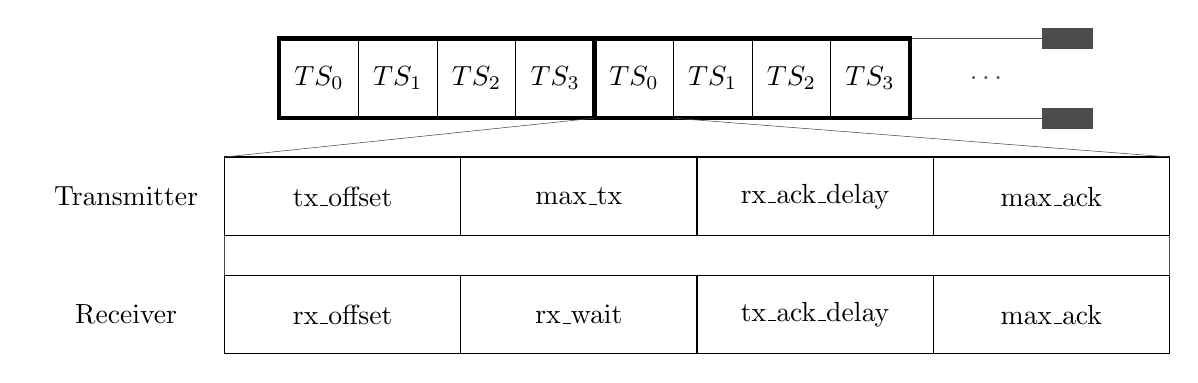
\begin{tikzpicture}[
  timeslot/.style={draw, rectangle, minimum size=1cm},
  description/.style={draw, rectangle, minimum size=1cm},
  arr/.style={help lines,black!70,<->},
]

\foreach [evaluate={\ts=int(mod(\i, 4))}] \i in {0,...,7} {
  \node (ts\i) [timeslot] at (\i, 0) {$TS_{\ts}$};
}
\node (ts8) [minimum height=1cm, minimum width=2cm, black!70] at (8.5, 0) {\ldots};

\draw[help lines, black!70]
  (ts8.north west) -- (ts8.north east) node[fill=white, black!70] {$\ldots$};
\draw[help lines, black!70]
  (ts8.south west) -- (ts8.south east) node[fill=white, black!70] {$\ldots$};

\draw[ultra thick] 
  (ts0.south west) rectangle (ts3.north east)
  (ts4.south west) rectangle (ts7.north east);

\begin{scope}[xshift=-1.2cm,yshift=-2cm,inner sep=0pt, outer sep=0pt]
  \node (desc) [fit={(-2.5,0) (0,1)}, label=center:{Transmitter}] {};
  \node (desc0) [description, fit={(0,0) (3,1)}, label=center:{tx\_offset}] {};
  \node (desc1) [description, fit={(3,0) (6,1)}, label=center:{max\_tx}] {};
  \node (desc2) [description, fit={(6,0) (9,1)}, label=center:{rx\_ack\_delay}] {};
  \node (desc3) [description, fit={(9,0) (12,1)}, label=center:{max\_ack}] {};
\end{scope}

\draw[help lines, black!70,-]
  ([yshift=0pt]ts4.south west) -- 
  ([yshift=0pt]{desc0.north west});
\draw[help lines, black!70,-]
  ([yshift=0pt]ts4.south east) -- 
  ([yshift=0pt]{desc3.north east});

\begin{scope}[xshift=-1.2cm,yshift=-3.5cm,inner sep=0pt, outer sep=0pt]
  \node (ddesc) [fit={(-2.5,0) (0,1)}, label=center:{Receiver}] {};
  \node (ddesc0) [description, fit={(0,0) (3,1)}, label=center:{rx\_offset}] {};
  \node (ddesc1) [description, fit={(3,0) (6,1)}, label=center:{rx\_wait}] {};
  \node (ddesc2) [description, fit={(6,0) (9,1)}, label=center:{tx\_ack\_delay}] {};
  \node (ddesc3) [description, fit={(9,0) (12,1)}, label=center:{max\_ack}] {};
\end{scope}

\draw[help lines, black!70,-]
  ([yshift=0pt]desc0.south west) -- 
  ([yshift=0pt]{ddesc0.north west});
\draw[help lines, black!70,-]
  ([yshift=0pt]desc3.south east) -- 
  ([yshift=0pt]{ddesc3.north east});
\end{tikzpicture}
}

\end{column}
\end{columns}
\end{frame}

\begin{frame}{Realization}
\framesubtitle{Adapt TSCH for LoRa}
\begin{columns}
\begin{column}{0.5\textwidth}
Hardware specific issues
\begin{itemize}
    \item Physical delay of RN2483
    \begin{itemize}
      \item No documentation
      \item Approximation
    \end{itemize}
    \only<2->{
      \item Missing feature
      \begin{itemize}
        \item Less precision
        \item Drift issues
      \end{itemize}
    }
\end{itemize}
\end{column}
\begin{column}{0.5\textwidth}

\resizebox{5.2cm}{3.4cm}{%
\begin{tikzpicture}[
  timeslot/.style={draw, rectangle, minimum size=1cm},
  description/.style={draw, rectangle, minimum size=1cm},
  arr/.style={help lines,black!70,<->},
]

\foreach [evaluate={\ts=int(mod(\i, 4))}] \i in {0,...,3} {
  \node (ts\i) [timeslot] at (\i, 0) {$TS_{\ts}$};
}
\node (ts4) [minimum height=1cm, minimum width=2cm, black!70] at (4.5, 0) {\ldots};
\draw[help lines, black!70]
  (ts4.north west) -- (ts4.north east) node[fill=white, black!70] {$\ldots$};
\draw[help lines, black!70]
  (ts4.south west) -- (ts4.south east) node[fill=white, black!70] {$\ldots$};

\draw[ultra thick] 
  (ts0.south west) rectangle (ts3.north east);

\begin{scope}[xshift=-1.2cm,yshift=-2.5cm,inner sep=0pt, outer sep=0pt]
  \node (desc) [draw,rectangle,fit={(0,0) (6,1)}, label=left:{Transmitter~}] {};
  \node (desc1) [description, fill=orange!20, fit={(3,0) (6,1)}, label=center:{data}] {};
  \node (desc0) [description, fill=gray!20, fit={(1,0) (3,1)}, label=center:{tx\_offset}] {};
  \node (desccont) [black!70, fit={(6,0) (8,1)}] {\ldots};
  \draw[help lines, black!70]
    (desccont.north west) -- (desccont.north east) node[fill=white, black!70] {$\ldots$};
  \draw[help lines, black!70]
    (desccont.south west) -- (desccont.south east) node[fill=white, black!70] {$\ldots$};
  \only<1>{
    \draw[pattern=north west lines, pattern color=green!50] (2.6,0) rectangle (3,1);
  }
\end{scope}

\begin{scope}[xshift=-1.2cm,yshift=-4.5cm,inner sep=0pt, outer sep=0pt]
  \node (ddesc) [draw,rectangle,fit={(0,0) (6,1)}, label=left:{Receiver~}] {};
  \node (ddesc0) [description, fill=gray!20, fit={(1,0) (3,1)}, label=center:{rx\_offset}] {};
  \draw[pattern=north west lines, pattern color=orange!50] (3,0) rectangle (6,1);
  \node (ddesccont) [black!70, fit={(6,0) (8,1)}] {\ldots};
  \draw[help lines, black!70]
    (ddesccont.north west) -- (ddesccont.north east) node[fill=white, black!70] {$\ldots$};
  \draw[help lines, black!70]
    (ddesccont.south west) -- (ddesccont.south east) node[fill=white, black!70] {$\ldots$};
  \only<1>{
    \draw[pattern=north west lines, pattern color=green!50] (6,0) rectangle (6.4,1);
  }
\end{scope}

\only<1->{
\begin{scope}[xshift=-1.2cm,yshift=-6.5cm,inner sep=0pt, outer sep=0pt]
  \node (comment) [red!70, fit={(5,0) (7,1)}] {};
\end{scope}
}

\only<2->{
\begin{scope}[xshift=-1.2cm,yshift=-6.5cm,inner sep=0pt, outer sep=0pt]
  \node (comment) [red!70, fit={(5,0) (7,1)}] {No Ack};
  \draw[help lines, thick, red!70,->]
    ([yshift=0pt]{comment.north west}) --
    ([yshift=0pt]ddesc0.south east);
\end{scope}
}

\draw[help lines, black!70,-]
  (ts3.south west) -- 
  ({desc.north west});
\draw[help lines, black!70,-]
  (ts3.south east) -- 
  ([xshift=12pt]{desccont.north east});
\end{tikzpicture}
}
\end{column}
\end{columns}
\end{frame}

\begin{frame}{Validation}
\framesubtitle{Driver}
\begin{columns}
\begin{column}{0.5\textwidth}
\begin{itemize}
    \item Basic Ping-Pong example
    \item Driver controlled by MAC layer
    \begin{itemize}
      \item Fully working on Contiki
    \end{itemize}
\end{itemize}
\end{column}
\begin{column}{0.5\textwidth}
\begin{figure}[H]
\centering
\begin{sequencediagram}
\newthread{A}{Mote A}{}
\newinst[1]{B}{Mote B}{}

\begin{call}[4]{A}{ping}{B}{pong}
\end{call}
\end{sequencediagram}
\end{figure}
\end{column}
\end{columns}
\end{frame}



\begin{frame}{Validation}
\framesubtitle{RPL}
\begin{figure}[H]
    \centering
    \resizebox{9.2cm}{4.5cm}{%
  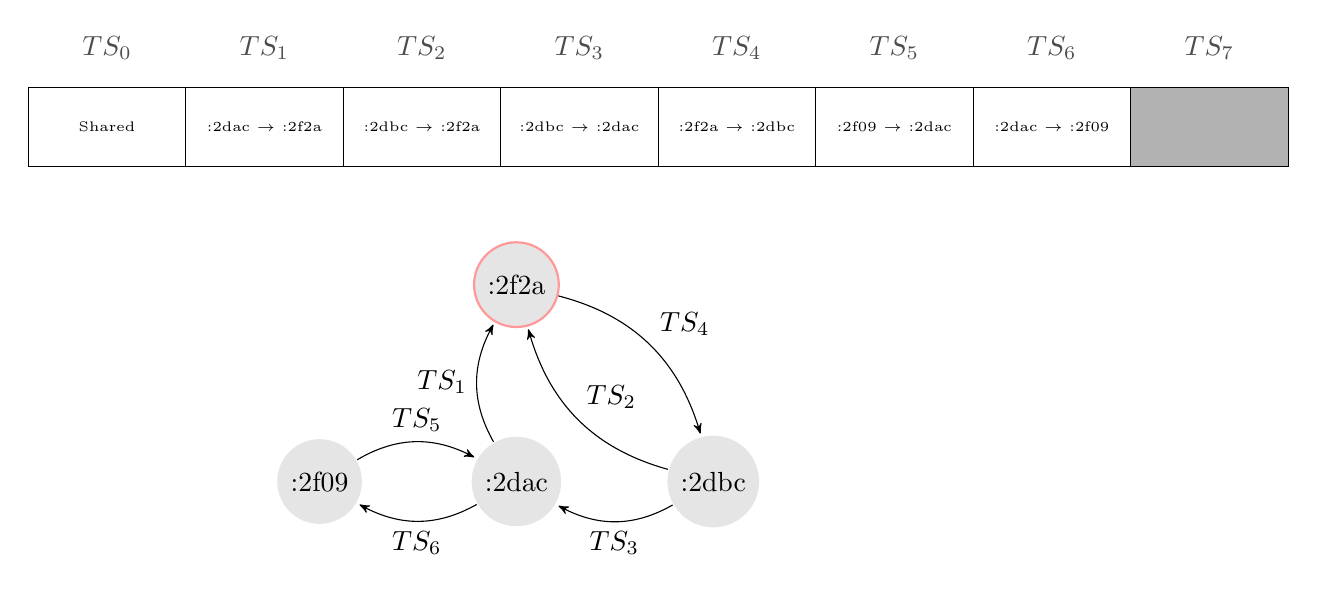
\begin{tikzpicture}[]

  \begin{scope}[
      xshift=-0.2cm,
      asn/.style={black!70, minimum width=2cm},
      timeslot/.style={draw, rectangle, minimum width=2cm, minimum height=1cm},
      arr/.style={help lines,black!70,<->},
  ]
    \foreach \i in {0,...,7} {
      \node (ts\i) [asn] at (2*\i, 1) {$TS_{\i}$};
    }
    \node (tss0) [timeslot] at (0, 0) {\tiny Shared};
    \node (tss1) [timeslot] at (2, 0) {\tiny :2dac $\rightarrow$ :2f2a};
    \node (tss2) [timeslot] at (4, 0) {\tiny :2dbc $\rightarrow$ :2f2a};
    \node (tss3) [timeslot] at (6, 0) {\tiny :2dbc $\rightarrow$ :2dac};
    \node (tss4) [timeslot] at (8, 0) {\tiny :2f2a $\rightarrow$ :2dbc};
    \node (tss5) [timeslot] at (10, 0) {\tiny :2f09 $\rightarrow$ :2dac};
    \node (tss6) [timeslot] at (12, 0) {\tiny :2dac $\rightarrow$ :2f09};
    \node (tss7) [timeslot, fill=black!30] at (14, 0) {};
  \end{scope}
  \begin{scope}[xshift=5cm,yshift=-2cm,->,>=stealth',shorten >=1pt,auto,node distance=2.5cm]
    \tikzstyle{every state}=[thick,draw=gray!50,fill=gray!20,draw=none,text=black]

    \node[state,thick,draw=red!40]         (A) [] {:2f2a};
    \node[state]         (B) [below of=A]       {:2dac};
    \node[state]         (C) [right of=B]       {:2dbc};
    \node[state]         (D) [left of=B]       {:2f09};

    \path (A) edge [bend left] node {$TS_4$} (C)
          (B) edge [bend left] node {$TS_1$} (A)
              edge [bend left] node {$TS_6$} (D)
          (C) edge [bend left] node[above right] {$TS_2$} (A)
              edge [bend left] node {$TS_3$} (B)
          (D) edge [bend left] node {$TS_5$} (B);
  \end{scope}
\end{tikzpicture}
}
\caption{Custom Schedule\label{fig:customsched}}
\end{figure}
\end{frame}

\begin{frame}{Validation}
\framesubtitle{RPL}
\begin{figure}[H]
\centering
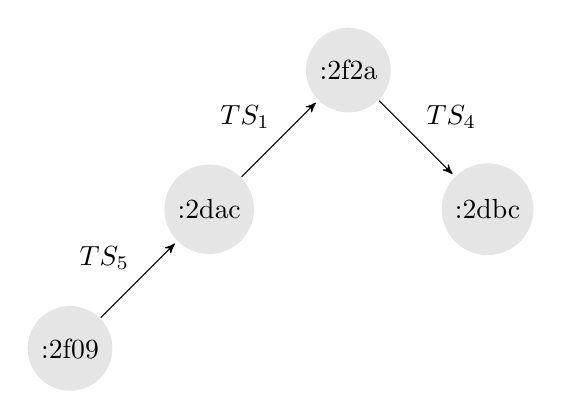
\begin{tikzpicture}[]

  \begin{scope}[xshift=5cm,yshift=-2cm,->,>=stealth',shorten >=1pt,auto,node distance=2.5cm]
    \tikzstyle{every state}=[thick,draw=gray!50,fill=gray!20,draw=none,text=black]

    \node[state]         (A) [] {:2f2a};
    \node[state]         (B) [below left of=A]       {:2dac};
    \node[state]         (C) [below right of=A]       {:2dbc};
    \node[state]         (D) [below left of=B]       {:2f09};

    \path (A) edge  node {$TS_4$} (C);
    \path (B) edge  node {$TS_1$} (A);
    \path (D) edge  node {$TS_5$} (B);
  \end{scope}
\end{tikzpicture}
\end{figure}
\end{frame}

\begin{frame}{Validation}
\framesubtitle{Jamming}
\begin{figure}[H]
\centering

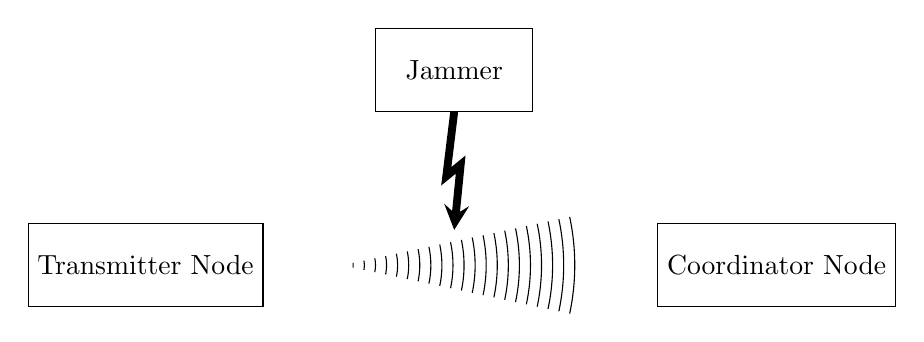
\begin{tikzpicture}[auto, node distance=2cm,>=latex']

\tikzset{
  block/.style = {draw, fill=white, rectangle, minimum height=3em, minimum width=2cm},
  input/.style = {coordinate},
  output/.style = {coordinate},
  pinstyle/.style = {pin edge={to-,t,black}},
  radiation/.style={decorate,decoration={expanding waves,angle=12,segment length=4pt}},
  zigzag/.style={to path={ -- ($(\tikztostart)!.55!-7:(\tikztotarget)$) -- ($(\tikztostart)!.45!7:(\tikztotarget)$) -- (\tikztotarget) \tikztonodes}}
}
\node[block](tx){Transmitter Node};
\node[block,above right= 2cm of tx](ttx){Jammer};
\node[block,right = 5cm of tx](rx){Coordinator Node};

\draw[radiation] ([shift={(1cm,0cm)}]tx.east)-- node [above=5mm] {} ([shift={(-1cm,0cm)}]rx.west);
\draw[-stealth,line width=1mm] (ttx.south) to[zigzag] +(0,-1.5);
\end{tikzpicture}

\caption{Structure of the channel jamming test\label{fig:jammer}}
\end{figure}
\end{frame}

\begin{frame}{Validation}
\framesubtitle{Jamming}
\begin{figure}[H]
  \centering
  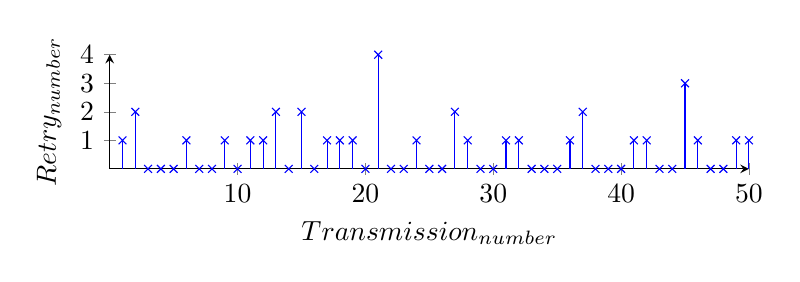
\begin{tikzpicture}

  \begin{groupplot}[group style={group size=1 by 2,
      horizontal sep=0pt,
      vertical sep=1cm},
      height=6cm,width=6cm,
  ]
  \nextgroupplot[
    ycomb,
    width=0.8\textwidth,
    height=0.25\textwidth,
    axis lines=middle,
    ymin=0,
    ymax=4,
    ylabel={$Retry_{number}$},
    ylabel near ticks,
    yticklabel style={/pgf/number format/1000 sep=},
    xmin=0,
    xmax=50,
    xlabel={$Transmission_{number}$},
    xlabel near ticks,
  ]
    \addplot[color=blue, mark=x] coordinates {
      (1,1)
      (2,2)
      (3,0)
      (4,0)
      (5,0)
      (6,1)
      (7,0)
      (8,0)
      (9,1)
      (10,0)
      (11,1)
      (12,1)
      (13,2)
      (14,0)
      (15,2)
      (16,0)
      (17,1)
      (18,1)
      (19,1)
      (20,0)
      (21,4)
      (22,0)
      (23,0)
      (24,1)
      (25,0)
      (26,0)
      (27,2)
      (28,1)
      (29,0)
      (30,0)
      (31,1)
      (32,1)
      (33,0)
      (34,0)
      (35,0)
      (36,1)
      (37,2)
      (38,0)
      (39,0)
      (40,0)
      (41,1)
      (42,1)
      (43,0)
      (44,0)
      (45,3)
      (46,1)
      (47,0)
      (48,0)
      (49,1)
      (50,1)
    };
  \end{groupplot}
  \end{tikzpicture}
  \caption{Retransmission per packet\label{fig:retransmission}}
\end{figure}
\end{frame}


\section{Conclusion}

{
  \setbeamercolor{background canvas}{bg=vubbleu}
  \setbeamercolor{normal text}{fg=white}
  \usebeamercolor*{normal text}
\begin{frame}[c]{}
  \centering
  \LARGE
  \vubfont
  ~Conclusion
\end{frame}
}

\begin{frame}{Conclusion}
\framesubtitle{}

\begin{itemize}
  \item
\end{itemize}

\end{frame}


{
  \setbeamercolor{background canvas}{bg=vubbleu}
  \setbeamercolor{normal text}{fg=white}
  \usebeamercolor*{normal text}
\begin{frame}[c]{}
  \centering
  \LARGE
  \vubfont
  ~Questions
\end{frame}
}

\begin{frame}{++}
\framesubtitle{Further Research}
\begin{itemize}
  \item Re-implementation on SX1272
  \begin{itemize}
    \item Optimize TSCH parameters
    \item EB interval
    \item Capacity measurement
    \item Radio Usage
  \end{itemize}
  \item Need digital analyser
  \begin{itemize}
    \item Measure TS drift precisely
    \item Latency
  \end{itemize}
\end{itemize}
\end{frame}

\begin{frame}{++}
\framesubtitle{TSCH - Related Work}
\begin{itemize}
    \item UWB-TSCH
    \begin{itemize}
      \item Port for UWB Communications
    \end{itemize}
    \item TSCH-over-LoRa
    \begin{itemize}
      \item April 2020
      \item Port for SX1272 LoRa Radio Module
    \end{itemize}
\end{itemize}
\footcitetext{tschoverlora}
\footcitetext{uwbtsch}
\end{frame}

\begin{frame}{++}
\framesubtitle{Time Slot}

\resizebox{11.2cm}{3.8cm}{%
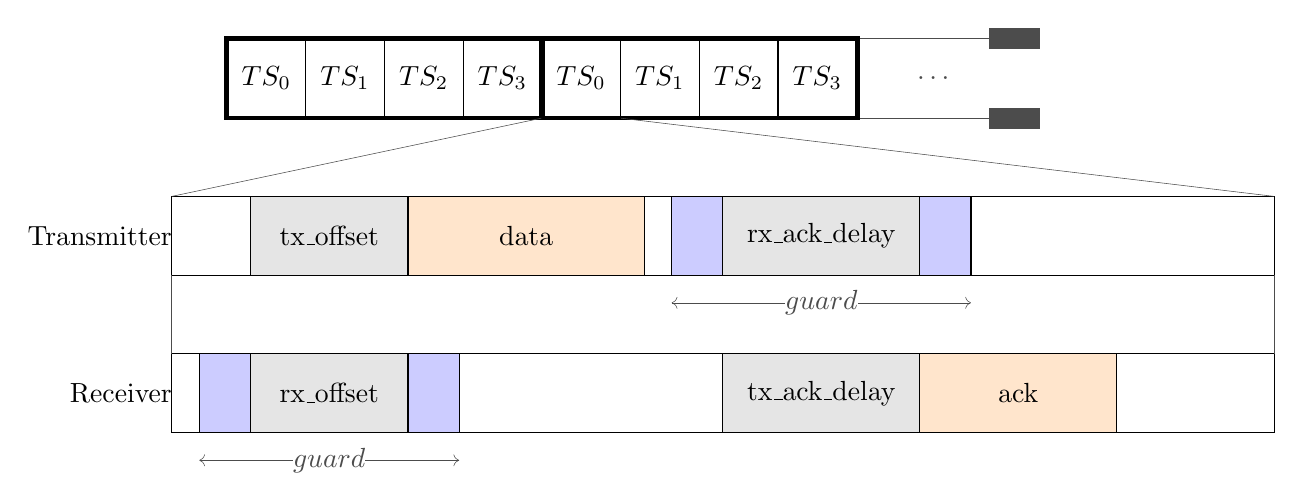
\begin{tikzpicture}[
  timeslot/.style={draw, rectangle, minimum size=1cm},
  description/.style={draw, rectangle, minimum size=1cm},
  arr/.style={help lines,black!70,<->},
]

\foreach [evaluate={\ts=int(mod(\i, 4))}] \i in {0,...,7} {
  \node (ts\i) [timeslot] at (\i, 0) {$TS_{\ts}$};
}
\node (ts8) [minimum height=1cm, minimum width=2cm, black!70] at (8.5, 0) {\ldots};

\draw[help lines, black!70]
  (ts8.north west) -- (ts8.north east) node[fill=white, black!70] {$\ldots$};
\draw[help lines, black!70]
  (ts8.south west) -- (ts8.south east) node[fill=white, black!70] {$\ldots$};

\draw[ultra thick] 
  (ts0.south west) rectangle (ts3.north east)
  (ts4.south west) rectangle (ts7.north east);

\begin{scope}[xshift=-1.2cm,yshift=-2.5cm,inner sep=0pt, outer sep=0pt]
  \node (desc) [draw,rectangle,fit={(0,0) (14,1)}, label=left:{Transmitter~}] {};
  \node (desc1) [description, fill=orange!20, fit={(3,0) (6,1)}, label=center:{data}] {};
  \node (desc0) [description, fill=gray!20, fit={(1,0) (3,1)}, label=center:{tx\_offset}] {};
  \node (descsync1) [description, fill=blue!20, fit={(6.7,0) (7,1)}] {};
  \node (descsync2) [description, fill=blue!20, fit={(9.5,0) (9.8,1)}] {};
  \node (desc2) [description, fill=gray!20, fit={(7,0) (9.5,1)}, label=center:{rx\_ack\_delay}] {};
  \draw[arr,<->]
      ([yshift=-10pt]descsync1.south west) -- node[fill=white] {$guard$} ([yshift=-10pt]{descsync2.south east});
\end{scope}

\draw[help lines, black!70,-]
  ([yshift=0pt]ts4.south west) -- 
  ([yshift=0pt]{desc.north west});
\draw[help lines, black!70,-]
  ([yshift=0pt]ts4.south east) -- 
  ([yshift=0pt]{desc.north east});

\begin{scope}[xshift=-1.2cm,yshift=-4.5cm,inner sep=0pt, outer sep=0pt]
  \node (ddesc) [draw,rectangle,fit={(0,0) (14,1)}, label=left:{Receiver~}] {};
  \node (ddescsync1) [description, fill=blue!20, fit={(0.7,0) (1,1)}] {};
  \node (ddescsync2) [description, fill=blue!20, fit={(3,0) (3.3,1)}] {};
  \node (ddesc0) [description, fill=gray!20, fit={(1,0) (3,1)}, label=center:{rx\_offset}] {};
  \draw[arr,<->]
      ([yshift=-10pt]ddescsync1.south west) -- node[fill=white] {$guard$} ([yshift=-10pt]{ddescsync2.south east});
  \node (ddesc2) [description, fill=gray!20, fit={(7,0) (9.5,1)}, label=center:{tx\_ack\_delay}] {};
  \node (ddesc3) [description, fill=orange!20, fit={(9.5,0) (12,1)}, label=center:{ack}] {};
\end{scope}

\draw[help lines, black!70,-]
    (desc.south west) -- ({ddesc.north west});
\draw[help lines, black!70,-]
    (desc.south east) -- ({ddesc.north east});
\end{tikzpicture}
}
\end{frame}

\begin{frame}{++}
\framesubtitle{Hardware Delay}

\resizebox{11.2cm}{3.8cm}{%
\begin{tikzpicture}[
  timeslot/.style={draw, rectangle, minimum size=1cm},
  description/.style={draw, rectangle, minimum size=1cm},
  arr/.style={help lines,black!70,<->},
]

\foreach [evaluate={\ts=int(mod(\i, 4))}] \i in {0,...,7} {
  \node (ts\i) [timeslot] at (\i, 0) {$TS_{\ts}$};
}
\node (ts8) [minimum height=1cm, minimum width=2cm, black!70] at (8.5, 0) {\ldots};

\draw[help lines, black!70]
  (ts8.north west) -- (ts8.north east) node[fill=white, black!70] {$\ldots$};
\draw[help lines, black!70]
  (ts8.south west) -- (ts8.south east) node[fill=white, black!70] {$\ldots$};

\draw[ultra thick] 
  (ts0.south west) rectangle (ts3.north east)
  (ts4.south west) rectangle (ts7.north east);

\begin{scope}[xshift=-1.2cm,yshift=-2.5cm,inner sep=0pt, outer sep=0pt]
  \node (desc) [draw,rectangle,fit={(0,0) (14,1)}, label=left:{Transmitter~}] {};
  \node (desc1) [description, fill=orange!20, fit={(3,0) (6,1)}, label=center:{data}] {};
  \node (desc0) [description, fill=gray!20, fit={(1,0) (3,1)}, label=center:{tx\_offset}] {};
  \node (descsync1) [description, fill=blue!20, fit={(6.7,0) (7,1)}] {};
  \node (descsync2) [description, fill=blue!20, fit={(9.5,0) (9.8,1)}] {};
  \node (desc2) [description, fill=gray!20, fit={(7,0) (9.5,1)}, label=center:{rx\_ack\_delay}] {};
  \draw[pattern=north west lines, pattern color=green!50] (2.6,0) rectangle (3,1);
\end{scope}

\draw[help lines, black!70,-]
  ([yshift=0pt]ts4.south west) -- 
  ([yshift=0pt]{desc.north west});
\draw[help lines, black!70,-]
  ([yshift=0pt]ts4.south east) -- 
  ([yshift=0pt]{desc.north east});

\begin{scope}[xshift=-1.2cm,yshift=-4.5cm,inner sep=0pt, outer sep=0pt]
  \node (ddesc) [draw,rectangle,fit={(0,0) (14,1)}, label=left:{Receiver~}] {};
  \node (ddescsync1) [description, fill=blue!20, fit={(0.7,0) (1,1)}] {};
  \node (ddescsync2) [description, fill=blue!20, fit={(3,0) (3.3,1)}] {};
  \node (ddesc0) [description, fill=gray!20, fit={(1,0) (3,1)}, label=center:{rx\_offset}] {};
  \node (ddesc2) [description, fill=gray!20, fit={(7,0) (9.5,1)}, label=center:{tx\_ack\_delay}] {};
  \node (ddesc3) [description, fill=orange!20, fit={(9.5,0) (12,1)}, label=center:{ack}] {};
  \draw[pattern=north west lines, pattern color=green!50] (6,0) rectangle (6.4,1);
\end{scope}

\draw[help lines, black!70,-]
    (desc.south west) -- ({ddesc.north west});
\draw[help lines, black!70,-]
    (desc.south east) -- ({ddesc.north east});
\end{tikzpicture}
}
\end{frame}




\end{document}

